\documentclass[a4paper,12pt]{article}

\usepackage[utf8]{inputenc}
\usepackage{geometry}

\geometry{
    left=1cm,
    right=1cm,
    top=1.5cm,
    bottom=2.5cm
}

\usepackage{setspace}
\usepackage{xcolor}
\usepackage{tikz}
\usepackage{tkz-graph}
\usetikzlibrary{trees}
\usetikzlibrary{arrows.meta} 

\definecolor{lightblue}{RGB}{124, 214, 235}
\definecolor{middleblue}{RGB}{38, 150, 201}
\definecolor{darkblue}{RGB}{49, 86, 148}

\begin{document}

    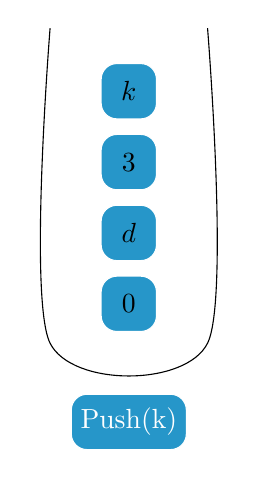
\begin{tikzpicture}[smooth, main/.style = {draw=white, text=black, fill=middleblue,  rounded corners=2mm, minimum size=2em}]
        \draw[x={(0cm,1cm)},y={(1cm,0cm)},color=black]
                plot coordinates{(4,1) (0,1) (0,3) (4,3)};
        \node[main] at (2, 0.5) {$0$};
        \node[main] at (2, 1.4) {$d$};
        \node[main] at (2, 2.3) {$3$};
        \node[main] at (2, 3.2) {$k$};
        \node[draw=white, text=white, fill=middleblue,  rounded corners=2mm, minimum size=2em] at (2, -1) {Push(k)};
    \end{tikzpicture}
    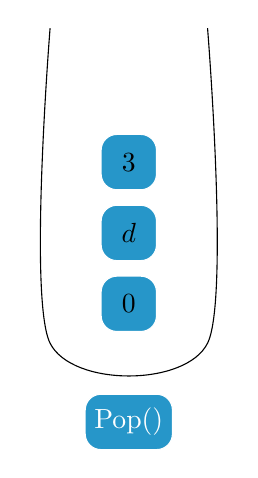
\begin{tikzpicture}[smooth, main/.style = {draw=white, text=black, fill=middleblue,  rounded corners=2mm, minimum size=2em}]
        \draw[x={(0cm,1cm)},y={(1cm,0cm)},color=black]
                plot coordinates{(4,1) (0,1) (0,3) (4,3)};
        \node[main] at (2, 0.5) {$0$};
        \node[main] at (2, 1.4) {$d$};
        \node[main] at (2, 2.3) {$3$};
        \node[draw=white, text=white, fill=middleblue,  rounded corners=2mm, minimum size=2em] at (2, -1) {Pop()};
    \end{tikzpicture}

    \begin{center}
        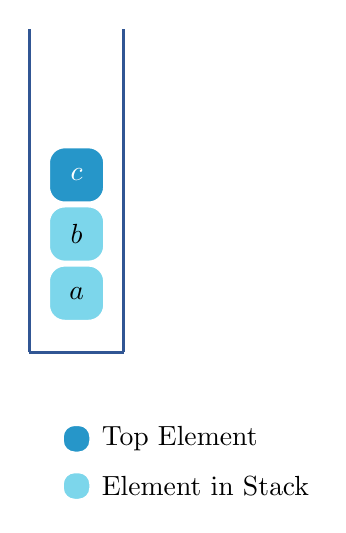
\begin{tikzpicture}[thick, 
            main/.style = {draw=white, text=black, fill=lightblue,rounded corners=2mm,minimum size=2em}, scale=0.2,
            selected/.style = {draw=white, text=white, fill=middleblue,rounded corners=2mm,minimum size=2em},
            EdgeStyle/.append style = {->, draw=darkblue, thick}]
            \matrix [column sep=0.1cm, row sep=0.02cm]{
            \node[selected] (3) {$c$};  \\ 
            \node[main] (2) {$b$};  \\ 
            \node[main] (1) {$a$};  \\ 
        };
        \draw[draw=darkblue,very thick] (-3,-7.5) -- (-3, 13);
        \draw[draw=darkblue,very thick] (3,-7.5) -- (3, 13);
        \draw[draw=darkblue,very thick] (-3,-7.5) -- (3, -7.5);

        \node[draw=white, text=white, fill=middleblue,rounded corners=1.5mm,minimum size=1em,label=right:Top Element] (A) at (0,-13) {}; % Distance between nodes: 3
        \node[draw=white, text=white, fill=lightblue,rounded corners=1.5mm,minimum size=1em,label=right:Element in Stack] (A) at (0,-16) {};
        \end{tikzpicture}
    \end{center}

    \vspace*{10mm}

    \begin{center}
        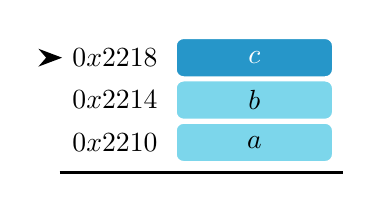
\begin{tikzpicture}[thick, scale=0.2,
            element/.style = {
                draw=white, 
                text=black, 
                fill=lightblue,
                rounded corners=1mm,
                minimum height=5mm,
                minimum width=20mm,
                }, 
            selected/.style = {
                draw=white, 
                text=white, 
                fill=middleblue,
                rounded corners=1mm,
                minimum height=5mm,
                minimum width=20mm}]
            \matrix [column sep=0.1cm, row sep=0.01cm]{
            \node[opacity=0] (sp) {}; & \node (999) {$0x2218$}; & \node[selected] {$c$};  \\ 
                                    & \node {$0x2214$}; & \node[element] {$b$};  \\ 
                                    & \node (A) {$0x2210$}; & \node[element] (B) {$a$};  \\ 
            };
            \draw[-{Stealth[length=3mm]}] (sp) -- (999);
            \draw (-8,-4.6) -- (10,-4.6);
            
        \end{tikzpicture}
    \end{center}

\end{document}